% Capítulo 8: bubble sort, estado do vetor ao fim de cada passada.
\documentclass[border=4pt]{standalone}
\usepackage[utf8]{inputenc}
\usepackage[T1]{fontenc}
% Estilo comum das figuras de vetores (capítulo 8).
\usepackage{tikz}
\usetikzlibrary{arrows.meta, positioning, calc, decorations.pathreplacing}
\definecolor{navy}{RGB}{23,45,80}
\definecolor{laranja}{RGB}{250,110,29}
\definecolor{cinzalogo}{RGB}{107,114,126}
\definecolor{azul}{RGB}{205,222,247}
\tikzset{
  casa/.style={draw=navy, line width=0.9pt, minimum width=8mm, minimum height=7mm,
               inner sep=0pt, font=\sffamily\small},
  pronta/.style={casa, fill=azul},
  parte/.style={casa, fill=laranja!12},
  marcada/.style={casa, fill=laranja!45, draw=laranja},
  fora/.style={casa, draw=cinzalogo!60, dashed, fill=white, text=cinzalogo!60},
  indice/.style={font=\sffamily\scriptsize, text=cinzalogo},
  explica/.style={font=\sffamily\small, text=navy, anchor=east},
  legenda/.style={font=\sffamily\scriptsize, text=cinzalogo},
  rotulo/.style={font=\sffamily\small\bfseries, text=navy},
  seta/.style={-{Stealth[length=2.2mm]}, navy, line width=0.9pt},
  chave/.style={decorate, decoration={brace, amplitude=4pt, mirror}, navy, line width=0.8pt},
}
% \vetor{nome}{x}{y}{valor/estilo, valor/estilo, ...}: casas lado a lado, chamadas nome0, nome1...
\newcommand{\vetor}[4]{%
  \foreach \valor/\estilo [count=\i from 0] in {#4} {
    \node[\estilo] (#1\i) at ($(#2, #3) + (\i*0.8, 0)$) {\valor};
  }
}

\begin{document}
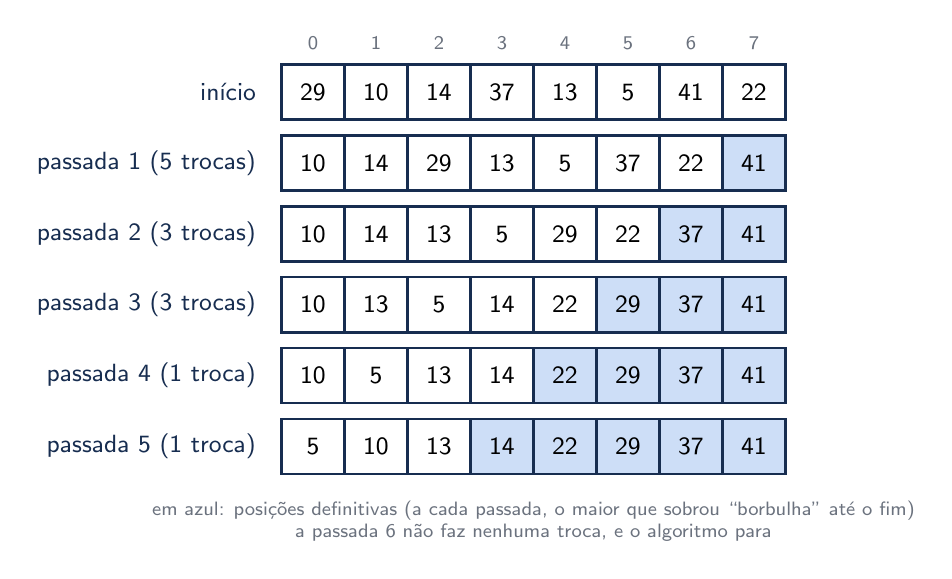
\begin{tikzpicture}
  \node[explica] at (-0.6, 0) {início};
  \vetor{a}{0}{0}{29/casa, 10/casa, 14/casa, 37/casa, 13/casa, 5/casa, 41/casa, 22/casa}
  \foreach \i in {0,...,7} { \node[indice, above=0.5mm of a\i] {\i}; }
  \node[explica] at (-0.6, -0.9) {passada 1 (5 trocas)};
  \vetor{b}{0}{-0.9}{10/casa, 14/casa, 29/casa, 13/casa, 5/casa, 37/casa, 22/casa, 41/pronta}
  \node[explica] at (-0.6, -1.8) {passada 2 (3 trocas)};
  \vetor{c}{0}{-1.8}{10/casa, 14/casa, 13/casa, 5/casa, 29/casa, 22/casa, 37/pronta, 41/pronta}
  \node[explica] at (-0.6, -2.7) {passada 3 (3 trocas)};
  \vetor{d}{0}{-2.7}{10/casa, 13/casa, 5/casa, 14/casa, 22/casa, 29/pronta, 37/pronta, 41/pronta}
  \node[explica] at (-0.6, -3.6) {passada 4 (1 troca)};
  \vetor{e}{0}{-3.6}{10/casa, 5/casa, 13/casa, 14/casa, 22/pronta, 29/pronta, 37/pronta, 41/pronta}
  \node[explica] at (-0.6, -4.5) {passada 5 (1 troca)};
  \vetor{f}{0}{-4.5}{5/casa, 10/casa, 13/casa, 14/pronta, 22/pronta, 29/pronta, 37/pronta, 41/pronta}
  \node[legenda, align=center] at (2.8, -5.45)
    {em azul: posições definitivas (a cada passada, o maior que sobrou ``borbulha'' até o fim)\\
     a passada 6 não faz nenhuma troca, e o algoritmo para};
\end{tikzpicture}
\end{document}
